\documentclass[conference]{IEEEtran}
\usepackage{amsmath}
\usepackage{textcomp}
\usepackage{cite}
\usepackage{graphicx}
\usepackage{booktabs}
\usepackage{array}
\usepackage{url}
\usepackage{subcaption}
\usepackage{breakurl}
\usepackage{epstopdf}
\usepackage{tabularx}
\usepackage{placeins}
\usepackage{float}
\usepackage{titlesec}
\usepackage{newtxtext}
\usepackage{newtxmath}

\titlespacing{\section}{0pt}{6pt}{4pt}
\titlespacing{\subsection}{0pt}{5pt}{3pt}
\titlespacing{\subsubsection}{0pt}{4pt}{2pt}

\title{GROUP\_14\_Experiment: 6\\Design of a Ring Oscillator Using IC7404 and CD4007 Transistors}

\author{
    \IEEEauthorblockA{Siddhant Shah (B23334) *, Akash Goel(B23032) †, 
                      Om Maheshwari (B23089) ‡, and Somya Bhadada (B23052) §}
* b23334@students.iitmandi.ac.in \\
† b23032@students.iitmandi.ac.in \\
‡ b23089@students.iitmandi.ac.in \\
§ b23052@students.iitmandi.ac.in}
\date{}

\begin{document}

\maketitle

\begin{abstract}
This paper presents the design methodology of a ring oscillator circuit using a IC7404 and CD4007 transistor and to observe its oscillatory behaviour.
\end{abstract}

\begin{IEEEkeywords}
Ring Oscillator, Propagation Delay, Oscillation Frequency, 74LS04, CD4007, Inverter Chain, Oscilloscope
\end{IEEEkeywords}



\section{Apparatus Required}
\begin{itemize}
    \item \textbf{74LS04 Hex Inverting Gates:} 
    \begin{itemize}
        \item Description: The 74LS04 is a digital logic device containing six independent NOT gates (inverters), each performing a logic inversion operation. It is commonly used in TTL logic circuits.
        \item Specifications: See Table~\ref{tab:74ls04_specs} for detailed electrical characteristics \cite{74LS04_Datasheet}.
        \begin{table}[h]
            \centering
            \begin{tabular}{ll}
                \toprule
                \textbf{Parameter} & \textbf{Value} \\
                \midrule
                Logic type & TTL \\
                Number of gates & 6 inverters \\
                Supply voltage (V\textsubscript{CC}) & 4.75V to 5.25V \\
                HIGH level input voltage (V\textsubscript{IH}) & Min 2V \\
                LOW level input voltage (V\textsubscript{IL}) & Max 0.8V \\
                HIGH level output current (I\textsubscript{OH}) & –0.4 mA \\
                LOW level output current (I\textsubscript{OL}) & 8 mA \\
                Propagation delay (t\textsubscript{PLH}/t\textsubscript{PHL}) & 3–15 ns \\
                Operating temperature range & 0°C to +70°C \\
                Package types & DIP, SOIC, SOP \\
                Power supply current (typical) & 1.2–6.6 mA depending on output state \\
                \bottomrule
            \end{tabular}
            \caption{74LS04 Hex Inverting Gate Specifications.}
            \label{tab:74ls04_specs}
        \end{table}
        \begin{figure}[h]
            \centering
            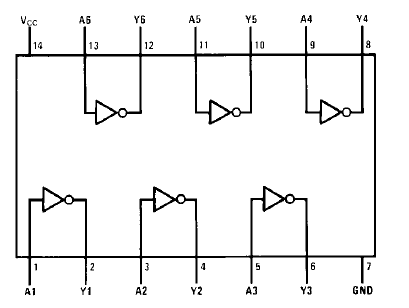
\includegraphics[width=0.3\textwidth]{74ls04_pinout.png} % Replace with actual image file
            \caption{74LS04 Pin Configuration (14-Pin DIP/SOIC/SOP).}
            \label{fig:74ls04_pinout}
        \end{figure}
    \end{itemize}

    \item \textbf{CD4007 CMOS Inverter configuration:}
    \begin{itemize}
        \item Description: A CMOS IC that includes three complementary pairs of N- and P-channel enhancement mode MOSFETs, suitable for logic-level switching and analog applications. All inputs are protected from static discharge by internal diode clamps.
        \item Specifications: See Table~\ref{tab:cd4007_specs} for detailed electrical characteristics \cite{CD4007_Datasheet}.
        \begin{table}[h]
            \centering
            \begin{tabular}{ll}
                \toprule
                \textbf{Parameter} & \textbf{Value} \\
                \midrule
                Supply voltage range (V\textsubscript{DD}) & 3V to 15V \\
                Operating temperature range & $-40^{\circ}$C to $+85^{\circ}$C \\
                Storage temperature range & $-65^{\circ}$C to $+150^{\circ}$C \\
                Maximum power dissipation (PDIP) & 700 mW \\
                Maximum power dissipation (SOIC) & 500 mW \\
                Quiescent current (I\textsubscript{L}) @ 5V & 0.005–15 µA \\
                Output drive (N-Channel) @ 10V & Up to 2.5 mA \\
                Output drive (P-Channel) @ 10V & Up to –2.5 mA \\
                Input capacitance & 5 pF \\
                Noise immunity (typ.) & 0.45 V\textsubscript{DD} \\
                Propagation delay @ 10V & 20–50 ns \\
                Transition time @ 10V & 30–50 ns \\
                Applications & Analog switches, logic inverters, digital design \\
                \bottomrule
            \end{tabular}
            \caption{CD4007C Electrical Specifications.}
            \label{tab:cd4007_specs}
        \end{table}
        \begin{figure}[h]
            \centering
            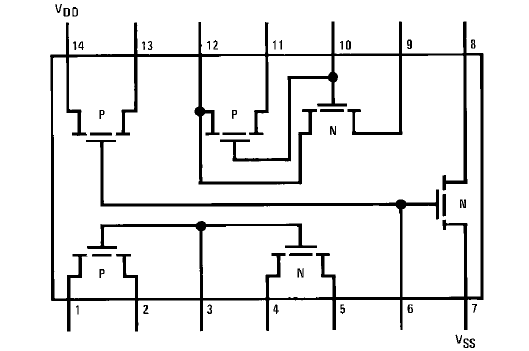
\includegraphics[width=0.3\textwidth]{cd4007_pinout.png} % Replace with actual image filename
            \caption{CD4007C Pin Configuration (DIP/SOIC).}
            \label{fig:cd4007_pinout}
        \end{figure}
    \end{itemize}

    \item \textbf{Power Supply:} Keithley 2231A-30-3 (triple output, 30V/3A).

    \item \textbf{DSO with Waveform Generator:} Keysight DSOX1102G (100 MHz, 1 GSa/s) for waveform analysis.

    \item \textbf{Breadboard and Connectors:} For circuit prototyping.
    
\end{itemize}


% Introduce the ring oscillator, experiment goals, components, and frequency formula.
\section{Introduction}
\noindent A \textbf{ring oscillator} is a circuit composed of an odd number of inverter stages connected in a feedback loop. The circuit lacks a stable logic state and continuously toggles between high and low states, producing a periodic oscillating signal. This behavior results from the inherent propagation delay of each inverter.

\noindent In this experiment, we construct ring oscillators using two different ICs—\textbf{74LS04} (TTL inverter) and \textbf{CD4007} (CMOS inverter). The goal is to compare their oscillation frequencies and understand how delay and inverter type affect the performance.

\noindent The frequency of oscillation is given by:
\begin{equation}
f = \frac{1}{2N\tau}
\end{equation}
where $N$ is the number of inverters and $\tau$ is the propagation delay per inverter.

% Explain the principles behind the ring oscillator’s operation and applications.
\section{Theory}
\noindent A ring oscillator operates due to the feedback of a signal through a chain of inverters. Each inverter introduces a delay, and with an odd number of stages, the signal continuously toggles, generating oscillations.

\subsection{Necessity of Odd Inverter Stages}
\noindent For the circuit to oscillate, the number of inverters in the loop must be odd. An even number of inverters would cancel out the inversion effect, resulting in a stable logic level. With an odd number, the feedback signal is always opposite in logic state, leading to continuous toggling due to delay.

\subsection{Frequency Determination Principles}
\noindent The total delay in the loop is $2N\tau$, accounting for rising and falling transitions. Thus, the frequency is:
\begin{equation}
f = \frac{1}{2N\tau}
\end{equation}
\noindent where:
\begin{itemize}
    \item $f$ = frequency of oscillation
    \item $N$ = number of inverters
    \item $\tau$ = propagation delay per inverter (depends on IC family)
\end{itemize}

\subsection{Advanced Applications}
\noindent Ring oscillators have several practical applications:
\begin{itemize}
    \item On-chip clock generation for digital circuits
    \item Measurement of gate delays and process variations
    \item Temperature and voltage monitoring circuits
    \item Random number generation (with noise injection)
\end{itemize}

% Describe circuit setup and theoretical frequency calculations.
\section{Design Calculations and Circuit Configuration}

\subsection{Design Calculations}
\noindent For a ring oscillator with 3 inverters, the frequency of oscillation is given by:
\begin{equation}
f = \frac{1}{2 \times 3 \times \tau} = \frac{1}{6\tau}
\end{equation}

\noindent Rearranging to find the propagation delay $\tau$:
\begin{equation}
\tau = \frac{1}{6f}
\end{equation}

\noindent The frequency $f$ will be measured using an oscilloscope connected to the output of the ring oscillator. Once the frequency is obtained, it is substituted into the above equation to calculate the propagation delay $\tau$ of each inverter.

\noindent For example:
\begin{itemize}
    \item If the measured frequency is $f = 10$ MHz, then:
    \[
    \tau = \frac{1}{6 \times 10 \times 10^6} = 16.67 \text{ ns}
    \]
\end{itemize}

\noindent This method allows us to experimentally determine the propagation delay of the inverter gates used (74LS04 or CD4007) based on the measured output frequency of the oscillator.


\subsection{Circuit Configuration}
\noindent The circuit consists of:
\begin{itemize}
    \item 3 inverter gates connected in a loop
    \item Output taken from any inverter stage
    \item Optional resistors or capacitors for shaping or measuring delay
\end{itemize}

\noindent \textbf{74LS04}: Connect pins of three inverters in a loop, power with +5V.  
\noindent \textbf{CD4007}: Use complementary NMOS and PMOS transistors to form three inverters. Power can range from +5V to +15V.

\begin{figure}[H]
\centering
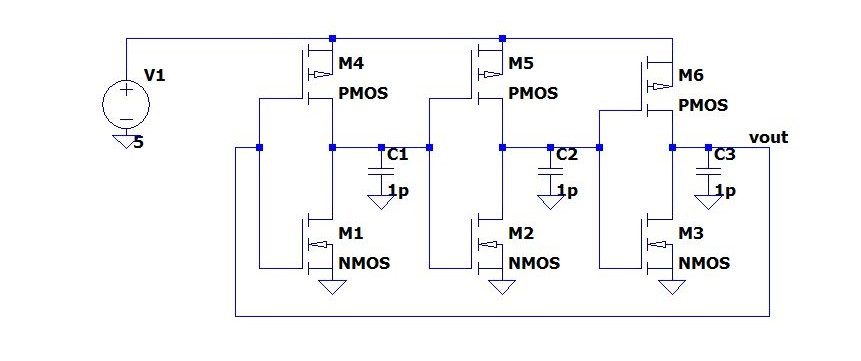
\includegraphics[width=0.4\textwidth]{ring_oscillator_CD4007.jpg}
\caption{Typical 3-stage ring oscillator configuration}
\label{fig:ring_oscillator}
\end{figure}

\section{Procedure}

\subsection{Part A: Using 74LS04 (TTL Inverter)}
\begin{enumerate}
    \item Connect the V\textsubscript{CC} pin (typically pin 14) of the 74LS04 IC to +5V and the GND pin (pin 7) to ground.
    \item Select three inverters from the six available in the 74LS04.
    \item Connect the output of the first inverter to the input of the second, and the output of the second to the input of the third.
    \item Feed the output of the third inverter back to the input of the first inverter to form a closed loop (ring).
    \item Observe the output waveform on an oscilloscope by probing the output of any one inverter.
    \item Measure the frequency of the oscillation using the oscilloscope’s frequency measurement tool.
    \item Use the frequency value in the formula \( \tau = \frac{1}{6f} \) to compute the propagation delay $\tau$.
\end{enumerate}

\begin{figure}[H]
\centering
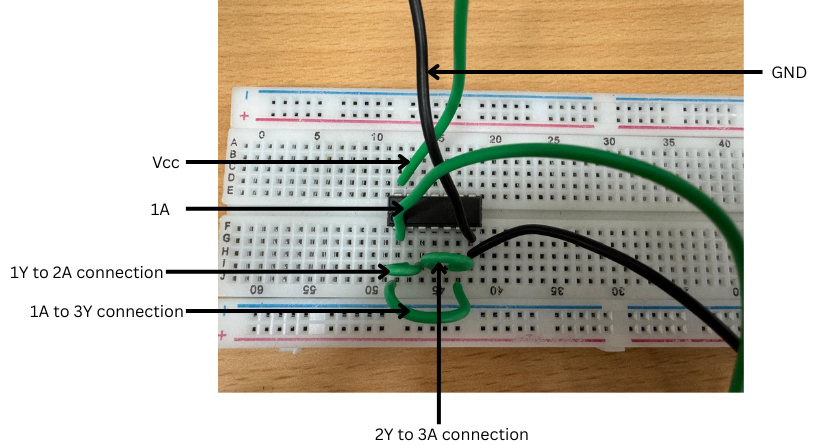
\includegraphics[width=1\columnwidth]{Circuit_74LS04.png}
\caption{Circuit implementation using 74LS04}
\label{fig:circuit_74LS04}
\end{figure}

\subsection{Part B: Using CD4007 (CMOS Inverter)}
\begin{enumerate}
    \item Connect the V\textsubscript{DD} pin (pin 14) of the CD4007 to +5V and the V\textsubscript{SS} pin (pin 7) to ground.
    \item Configure three CMOS inverters using the internal NMOS and PMOS transistors according to the CD4007 pinout.
    \item Connect the three inverters in a ring configuration: output of one inverter to the input of the next, and the last inverter back to the first.
    \item Observe the output waveform on an oscilloscope and measure its frequency.
    \item Calculate the propagation delay using the measured frequency: \( \tau = \frac{1}{6f} \).
\end{enumerate}

\begin{figure}[H]
\centering
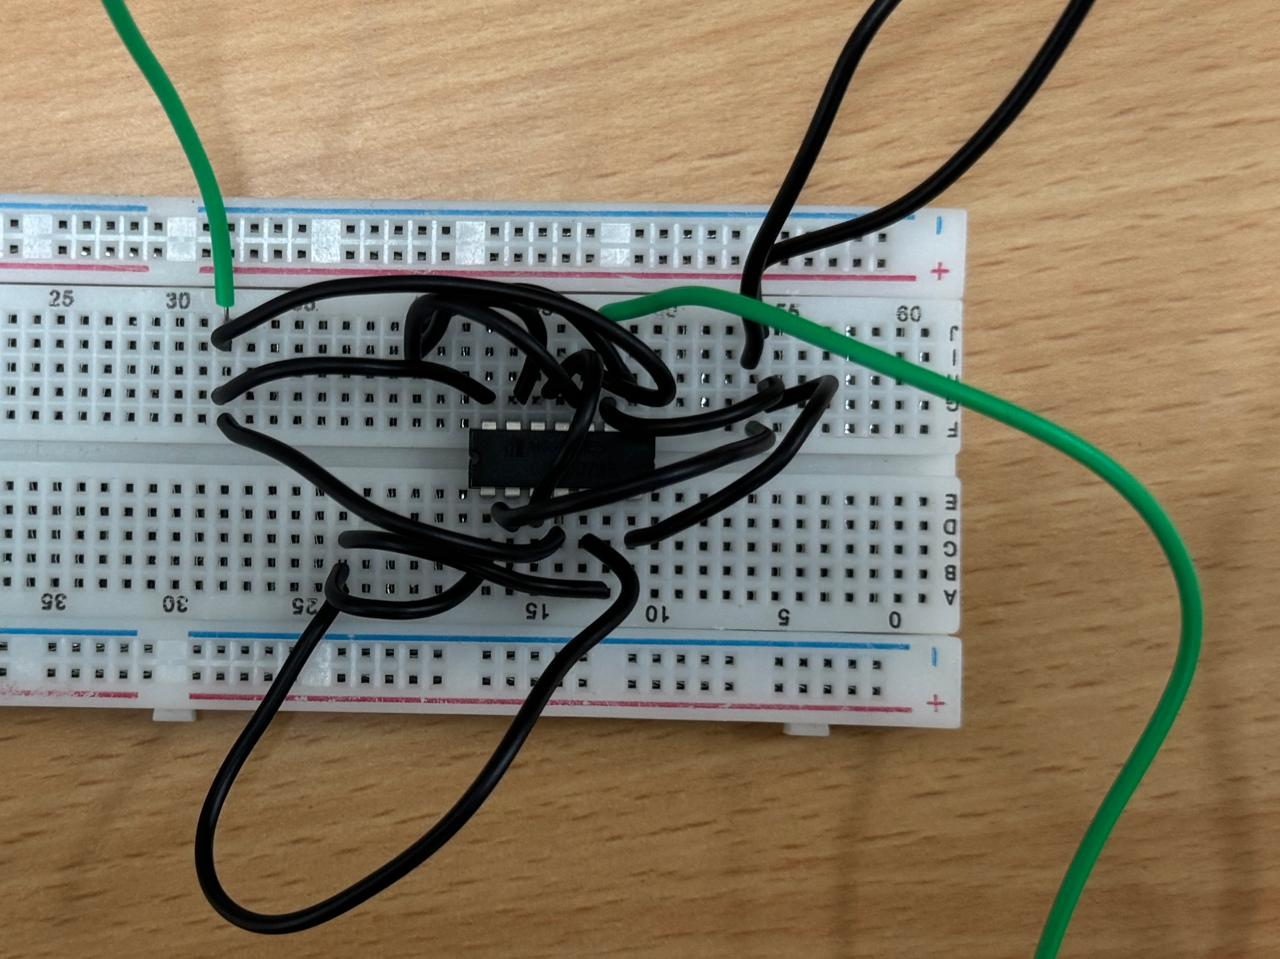
\includegraphics[width=0.7\columnwidth]{Circuit_CD4007.jpg}
\caption{Circuit implementation using CD4007}
\label{fig:circuit_CD4007}
\end{figure}


\section{Results and Observations}

\subsection{IC7404 Results}
\noindent The ring oscillator was constructed using three inverters from the 74LS04 IC. The output waveform was observed on the oscilloscope, and the frequency was measured.

\begin{itemize}
    \item Measured Frequency: \textbf{58 MHz}
    \item Theoretical Delay ($\tau$): 
    \begin{equation}
        \tau = \frac{1}{6f} = \frac{1}{6 \times 58 \times 10^6} \approx 2.9 \text{ ns}
    \end{equation}
    \item Observed waveform is nearly square with a consistent period, indicating stable oscillation.
\end{itemize}

\begin{figure}[H]
    \centering
    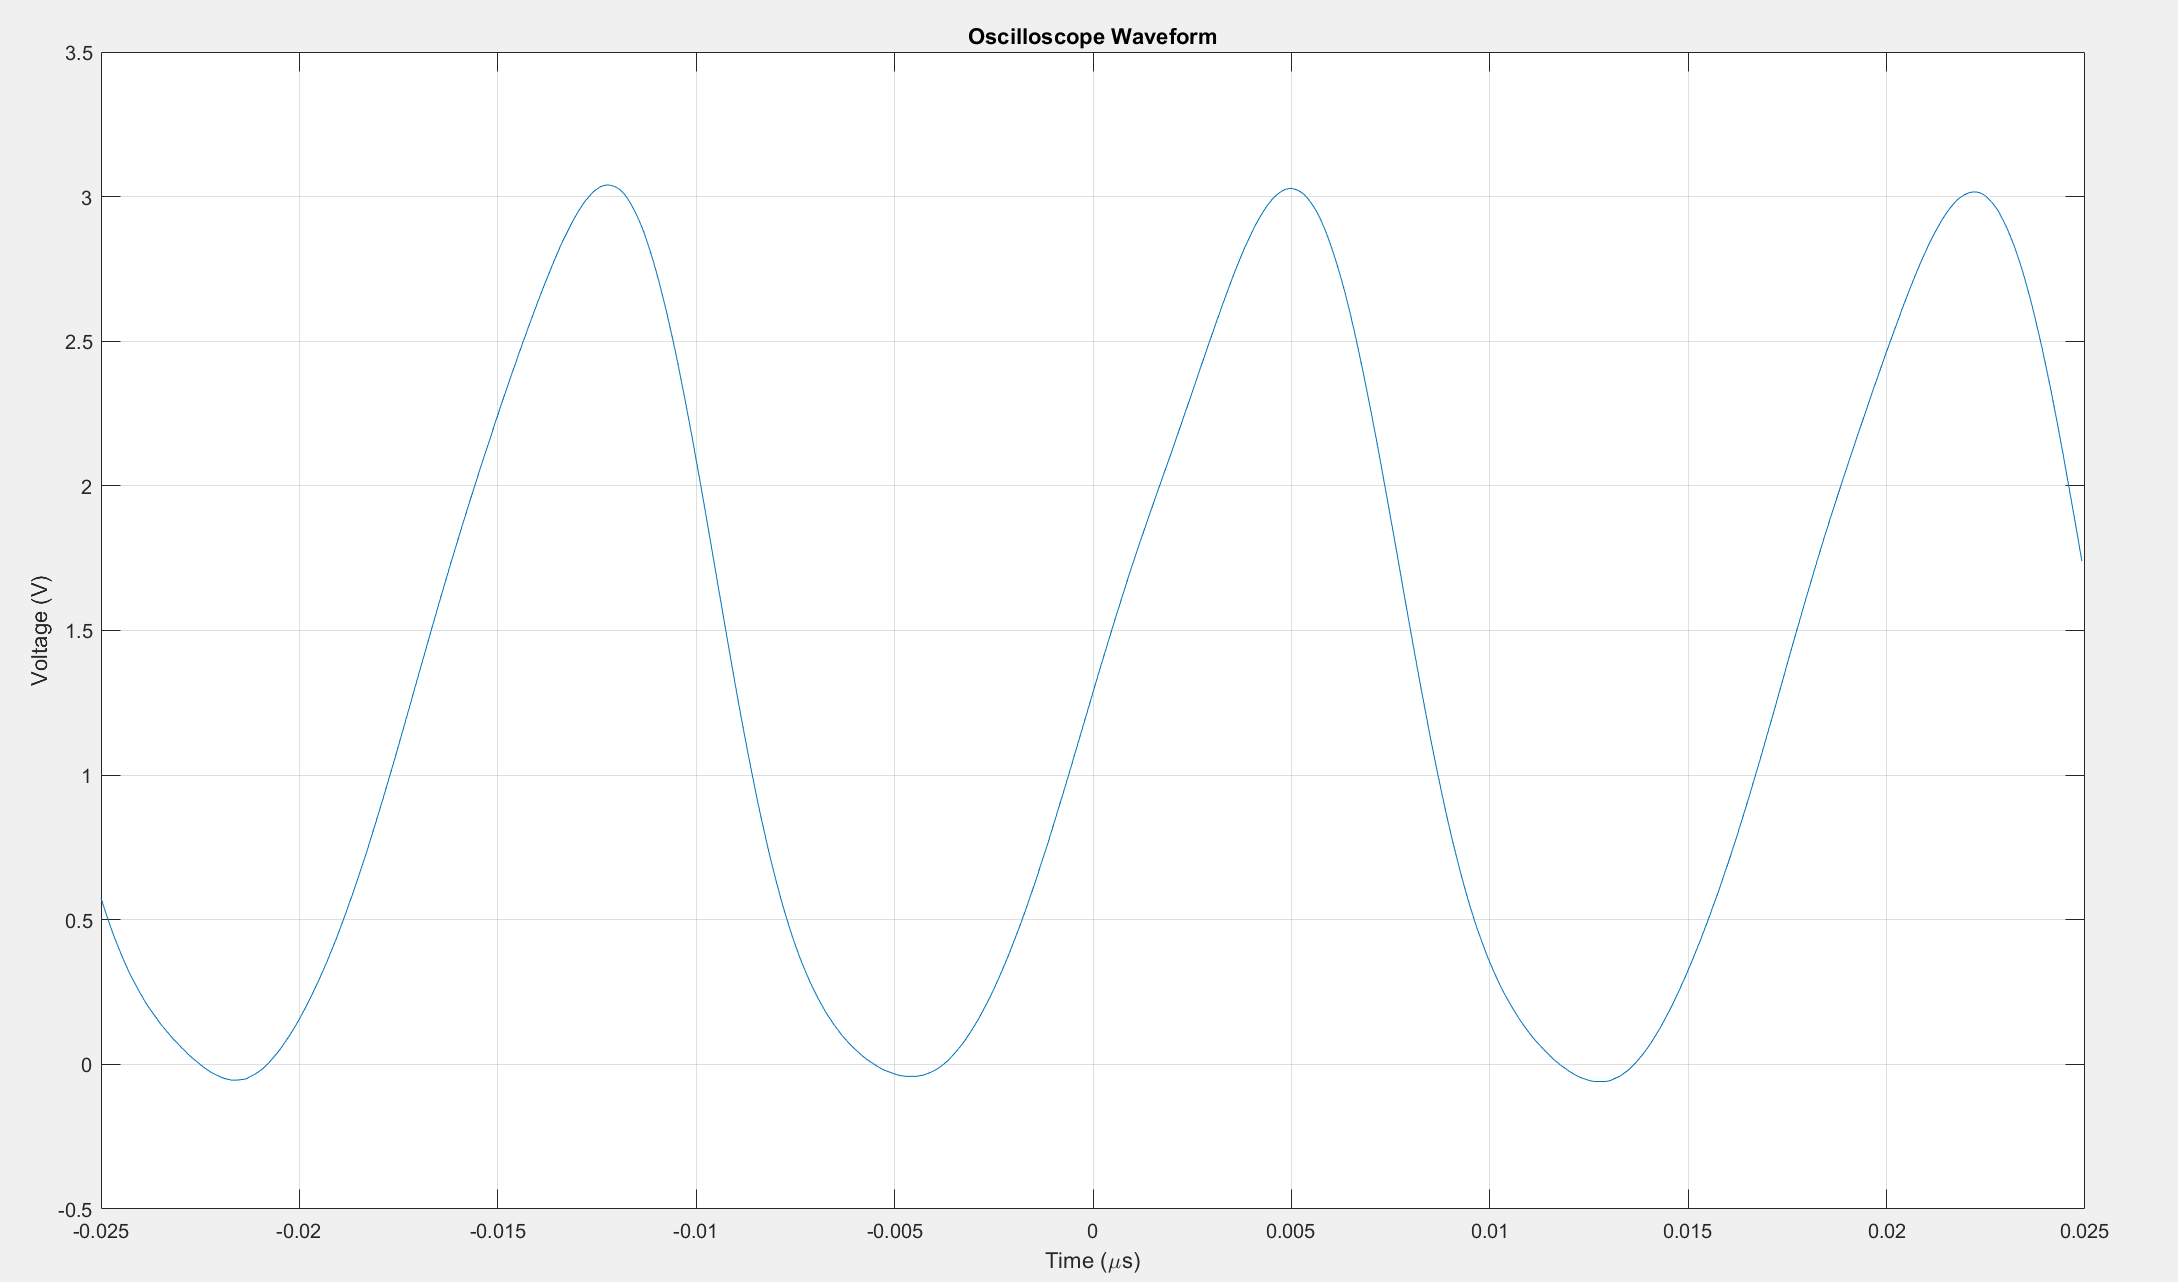
\includegraphics[width=\columnwidth]{IC7404_waveform.png}
    \caption{Oscilloscope output waveform of IC7404-based ring oscillator.}
    \label{fig:ic7404_waveform}
\end{figure}

\subsection{CD4007 Results}
\noindent The ring oscillator was also built using three CMOS inverters configured from the CD4007 IC. Frequency was similarly measured using an oscilloscope.

\begin{itemize}
    \item Measured Frequency: \textbf{50 MHz}
    \item Theoretical Delay ($\tau$): 
    \begin{equation}
        \tau = \frac{1}{6f} = \frac{1}{6 \times 50 \times 10^6} \approx 2.8 \text{ ns}
    \end{equation}
    \item The waveform was slightly slower in transition due to the higher propagation delay of CMOS technology.
\end{itemize}

\begin{figure}[H]
    \centering
    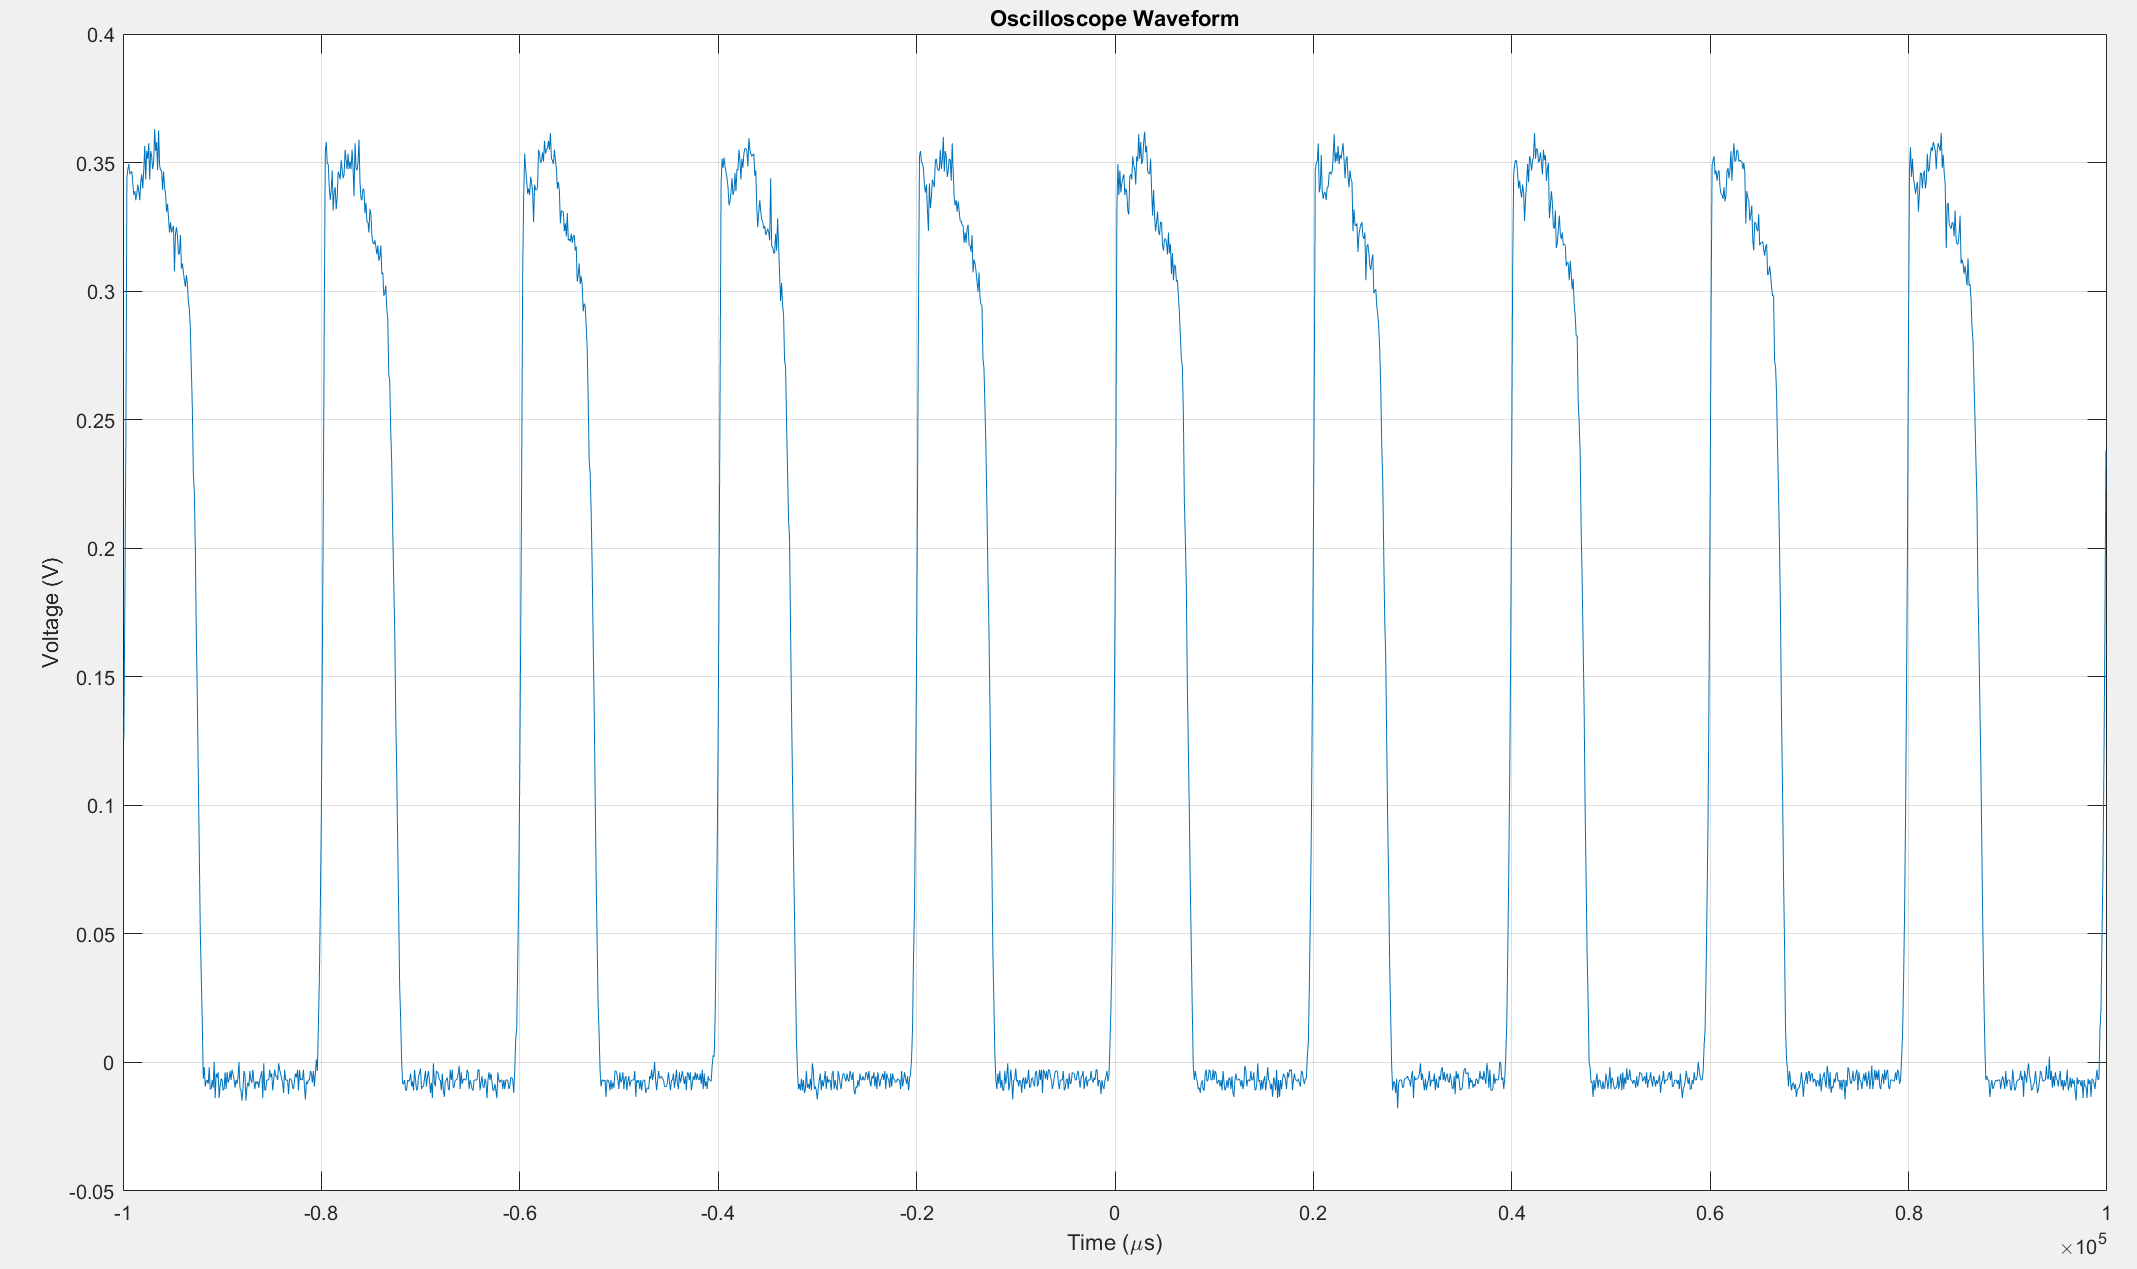
\includegraphics[width=\columnwidth]{CD4007_waveform.png}
    \caption{Oscilloscope output waveform of CD4007-based ring oscillator.}
    \label{fig:cd4007_waveform}
\end{figure}

\begin{figure}[H]
    \centering
    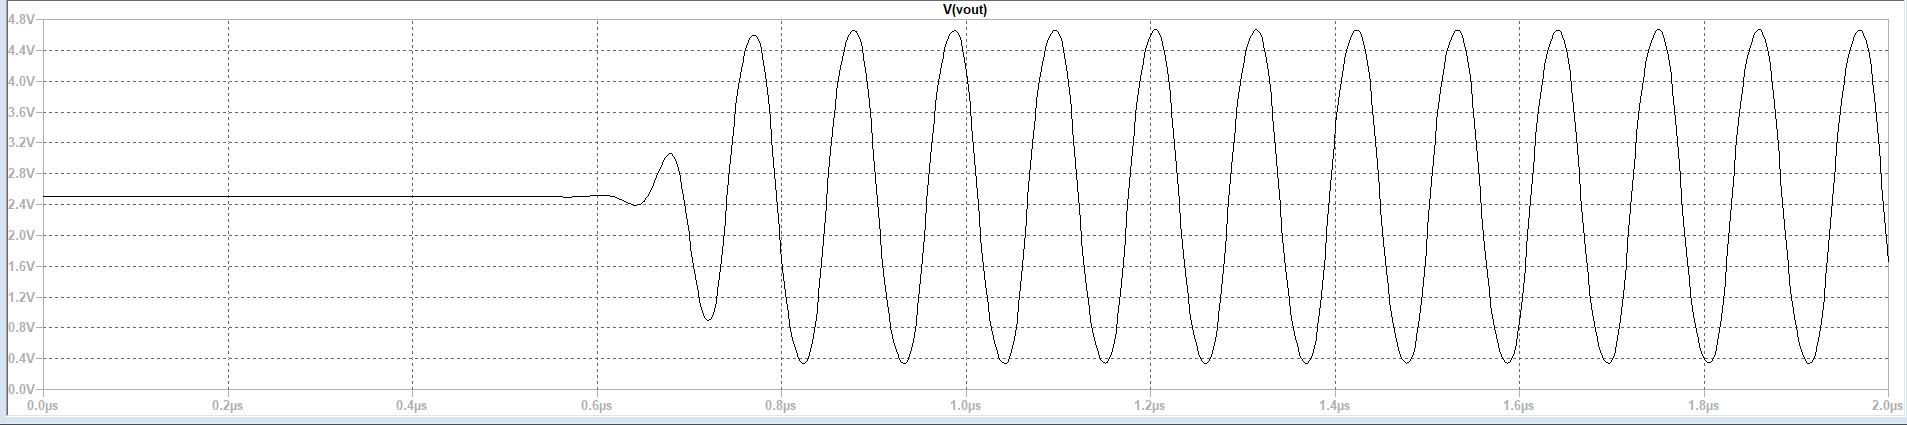
\includegraphics[width=\columnwidth]{CD4007_LTspice.jpg}
    \caption{LTSpice output waveform of CD4007-based ring oscillator.}
    \label{fig:cd4007_waveform}
\end{figure}

\subsection{IC7404 Bonus Results}
\noindent The ring oscillator was constructed using five inverters from the 74LS04 IC. The output waveform was observed on the oscilloscope, and the frequency was measured.

\begin{itemize}
    \item Measured Frequency: \textbf{58 MHz}
    \item Theoretical Delay ($\tau$): 
    \begin{equation}
        \tau = \frac{1}{6f} = \frac{1}{6 \times 58 \times 10^6} \approx 2.9 \text{ ns}
    \end{equation}
    \item Observed waveform is nearly square with a consistent period, indicating stable oscillation.
\end{itemize}

\begin{figure}[H]
    \centering
    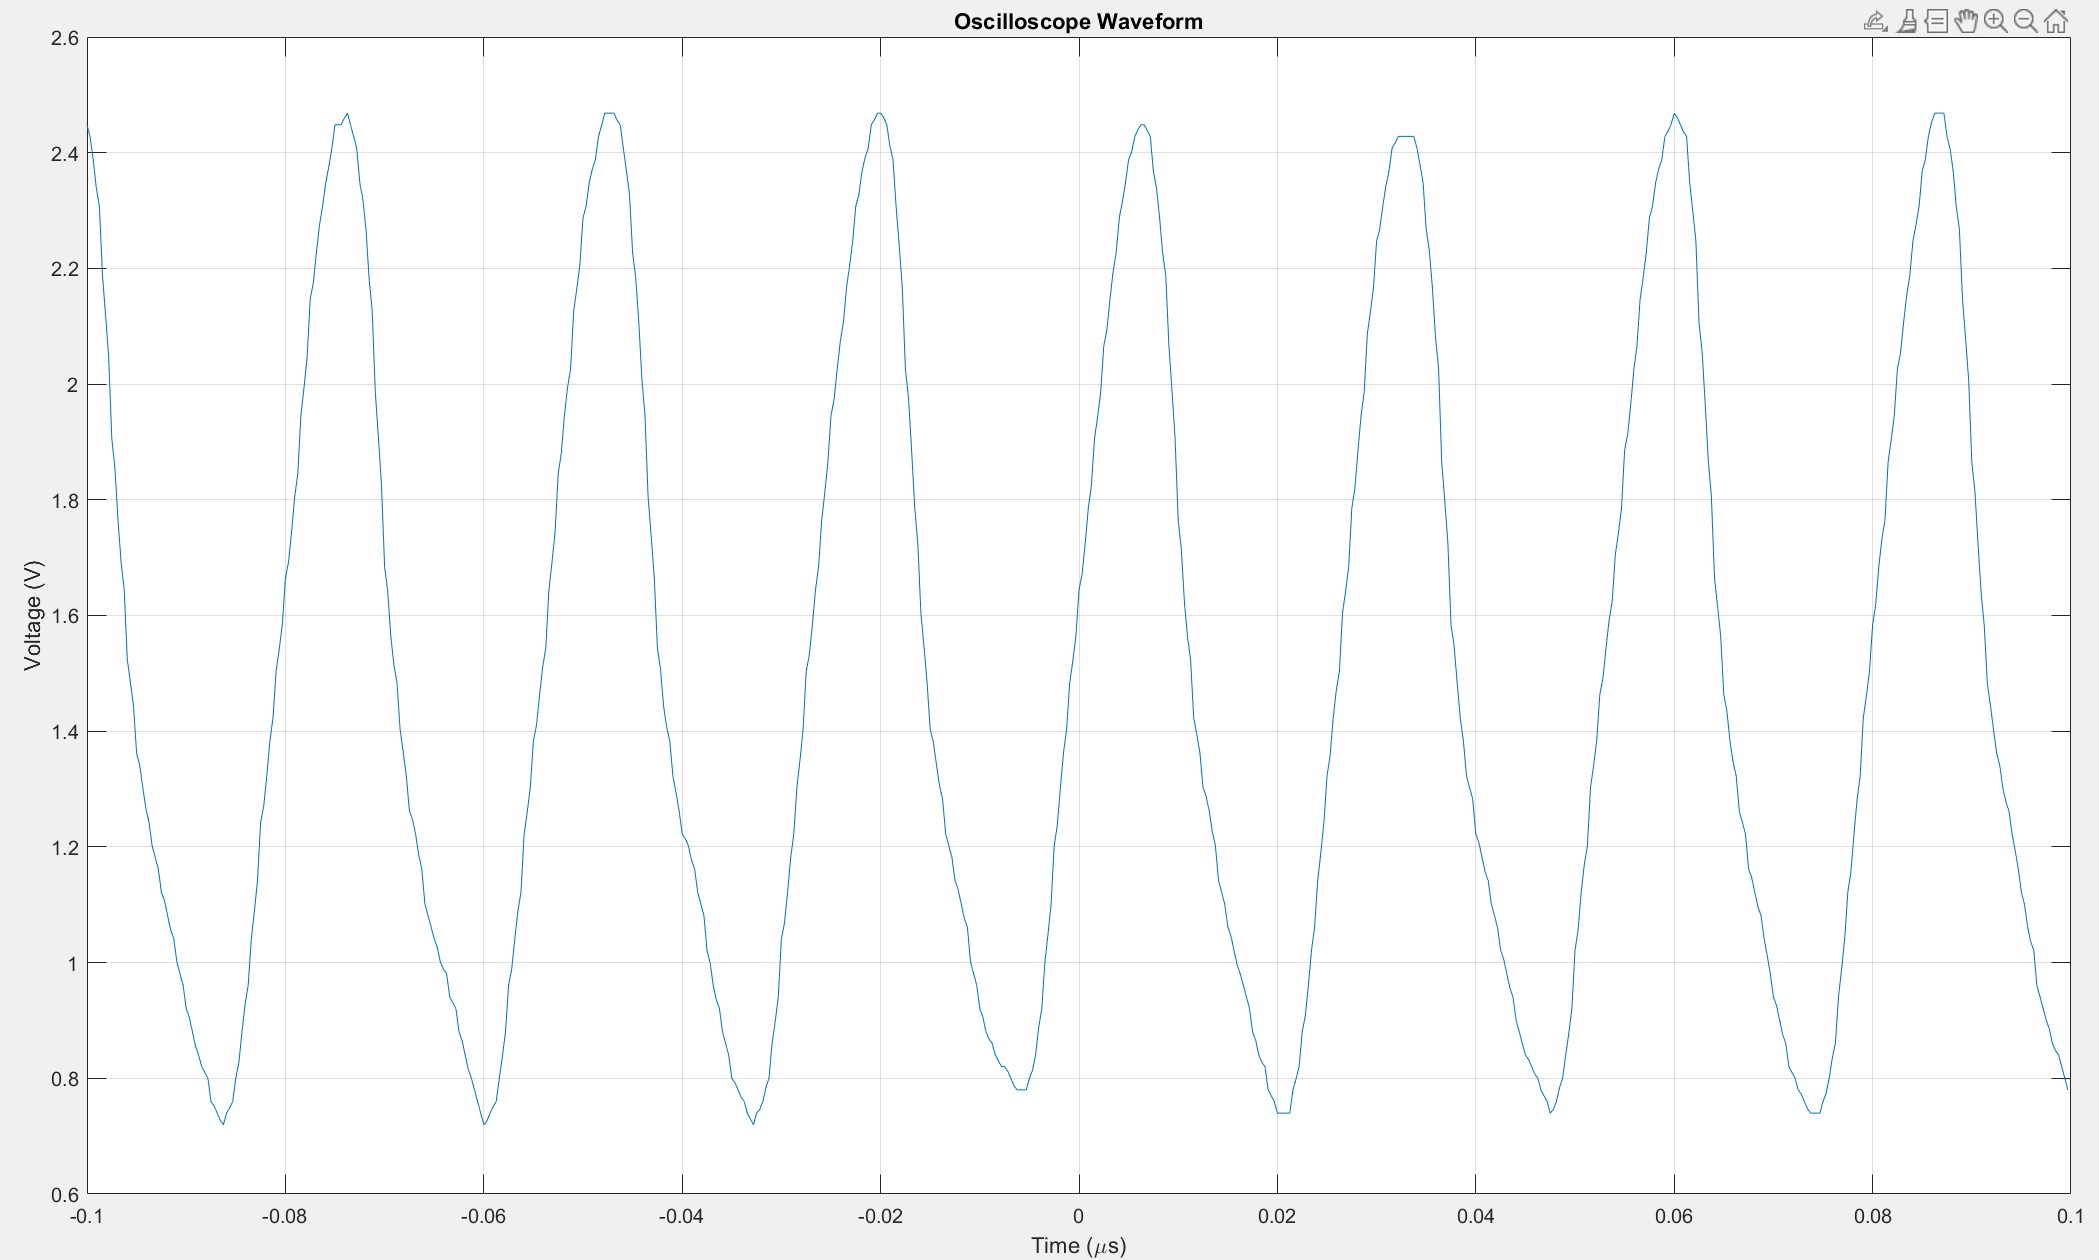
\includegraphics[width=\columnwidth]{IC7404_waveform_5.png}
    \caption{Oscilloscope output waveform of IC7404-based ring oscillator.}
    \label{fig:ic7404_waveform}
\end{figure}

\section{Conclusion}
\noindent The ring oscillator experiment was successfully implemented using two types of logic families: TTL (74LS04) and CMOS (CD4007). The output frequency of oscillation was measured using an oscilloscope, and corresponding propagation delays were calculated using the standard ring oscillator formula. Results showed that the TTL-based oscillator (with 74LS04) achieved a higher frequency due to lower gate delay compared to the CMOS-based oscillator (CD4007), which exhibited slower operation due to higher propagation delay. The observed results align well with theoretical expectations, validating the working principles of ring oscillators.

\noindent This experiment reinforced the importance of propagation delay in high-speed digital circuit design and demonstrated how the type of logic family directly impacts signal timing and oscillation characteristics.

\section{Practical Considerations}
\begin{itemize}
    \item Ensure that the power supply voltage levels are appropriate for each IC family: typically 5V for TTL (74LS04) and 5V–15V for CMOS (CD4007).
    \item Avoid floating inputs on unused gates to prevent noise and instability in oscillation.
    \item Use short and direct wiring on the breadboard to minimize parasitic capacitance and inductance, which could distort the waveform.
    \item Place the oscilloscope probe close to the output pin of the last inverter stage for accurate waveform capture.
    \item If the oscillator does not start, try using a high-value resistor (e.g., 10k$\Omega$) for feedback or adding capacitive loading at the output to help sustain oscillation.
    \item Ensure all inverter stages are connected properly in sequence with correct orientation to maintain the required odd number of inverters.
    \item Be cautious of signal degradation due to loading effects if driving external circuits directly from the oscillator output.
\end{itemize}


\begin{thebibliography}{9}
\bibitem{b1} A. S. Sedra and K. C. Smith, \textit{Microelectronic Circuits}, 7th ed., Oxford University Press, 2015.
\bibitem{b2} R. Boylestad and L. Nashelsky, \textit{Electronic Devices and Circuit Theory}, 11th ed., Pearson, 2013.

	
    \bibitem{Sedra_Smith}
    A. Sedra, K. Smith, \textit{Microelectronic Circuits}, 7th ed. Oxford University Press, 2014.

    \bibitem{Razavi_Fundamentals}
    B. Razavi, \textit{Fundamentals of Microelectronics}, 2nd ed. Wiley, 2013.

    \bibitem{74LS04_Datasheet} 
     Fairchild Semiconductor Corporation, "74LS04 Datasheet," 2000. [Online]. Available: \url{https://www.futurlec.com/74LS/74LS04.shtml}

    \bibitem{CD4007_Datasheet} 
     Fairchild Semiconductor Corporation, "CD4007 Datasheet," 1999. [Online]. Available: \url{https://www.futurlec.com/4000Series/CD4007.shtml}
    

\end{thebibliography}

\end{document}

